\documentclass[8pt]{article}
\usepackage{geometry}                % See geometry.pdf to learn the layout options. There are lots.
\geometry{letterpaper}                   % ... or a4paper or a5paper or ... 
%\geometry{landscape}                % Activate for for rotated page geometry
%\usepackage[parfill]{parskip}    % Activate to begin paragraphs with an empty line rather than an indent
\usepackage{graphicx}
\usepackage{amssymb}
\usepackage{epstopdf}
\usepackage{tipa}
\usepackage{amsmath}

\DeclareGraphicsRule{.tif}{png}{.png}{`convert #1 `dirname #1`/`basename #1 .tif`.png}
\graphicspath{{/Users/marlon/Documents/BA/thesis/pictures/}}

\title{Unsupervised Cognate Identification with Variational Autoencoders}
\author{Marlon Betz}
%\date{}                                           % Activate to display a given date or no date

\begin{document}
\maketitle
\newpage
\tableofcontents
\newpage

\section{Introduction}

Historical Linguistics investigates language from a diachronic perspective, i.e. it seeks to uncover the history of languages and the structure of the hidden forces that drive language change.  Computational Historical Linguistics accordingly deals with computational methods to explore the history of languages and topics closely related to it, such as phylogenetic inferences of language families \cite{bouckaert2012mapping}, migration of language speakers \cite{gray2009language}, inferring lexical flows between languages \cite{dellert2015uralic} or modeling sound change \cite{bouchard2013automated}.  

On the other hand, deep neural networks have been proven to uncover latent features of data and use them for a variety of tasks. Deep Autoencoders perform well on information retrieval tasks.


 However, Computation Historical Linguistics has hardly been touched yet by the current Deep Learning boom (a notable exception is \cite{rama2016siamese}). 
The aim of this thesis is hence 
\begin{enumerate}
\item to combine methods from both Computational Historical Linguistics and the emerging field of Deep Learning
\item to propose a model of modeling sound change as a walk in latent space, which is suitable for neural networks
\item to use variational autoencoders as a means to uncover the the latent structure that describes the connection between the phonological shape and the meaning of a given word, as well as the geographical location of the speakers of the language the word belongs to, and to investigate it
\item to show how this uncovered structure can be used to identify cognates in an unsupervised way
\end{enumerate}

I will first start by giving an overview of the problem of cognate identification and related fields of research. I will give a background on why cognate identification is important to discuss the historical connections between languages and further provide an overview on several established methods to detect cognates.  

Then I will proceed to introduce the concept of sound change as a walk in latent space, which serves as a background for the actual inference model. Here I will talk about the main motivations for this approach as well as its major drawbacks. 


I will then discuss the actual architecture of the inference model. This first covers a general overview on the components included in the model. I will then in detail look over all components in particular. That will first cover a discussion of different methods of phoneme vectorizations. This is followed by a general overview on autoencoders as non-linear dimensionality reduction architectures first and then a description of variational autoencoders in particular, which build the backbone of the model described here. I then come to the discussion of possible ways to cluster the words, i.e. to assign the actual inferred cognacy labels.

Then I will document how well those methods can be used to infer cognacy between words. I will compare the inferred labels with expert judgements first and then see how the inferred labels can infer language phylogenies, using established bayesian models of cognate evolution.

Finally, I will give a resume on the model described here.


\section{Sound Change as a Walk in Latent Space}
\label{Sound Change as a Walk in Latent Space}
\subsection{Motivation}

\begin{figure}[h]
\begin{center}
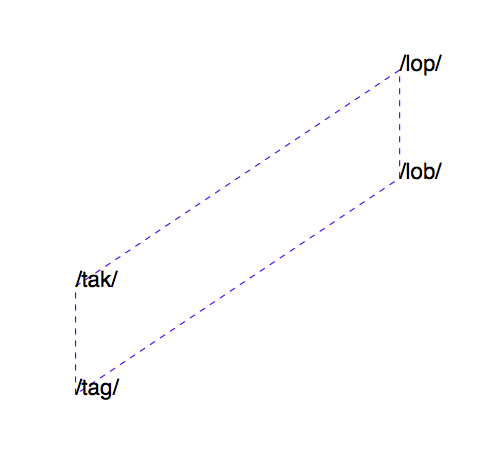
\includegraphics[width=0.5\textwidth]{sc_fake_example} 
\caption{Visualization of the concept of sound change as a walk in latent space. Here, sound changes are vectors from one word to another, where both word forms are given as points in latent space. The vector from /lob/ to /lop/ would be the same as from /tag/ to /tak/, as both vectors would describe the loss of voice in the word-final phoneme. This linear dependence means that if we fit a regression model from /tag/ to /tak/, we could generalize well to predict /lop/ from /lob/. The different lengths of the vectors are than proportional to probabilities of such as sound change to appear. Here, final devoicing should be more probable than a change from /lop/ to /tak/. }
\label{default}
\end{center}
\end{figure}
In linguistic literature, sound change is usually described as a change of distinctive phonological features over phonological symbols. For instance, a sound change such as final devoicing as in 

\begin{equation}
MHG /hund/ \rightarrow NHG /hunt/
\end{equation}

 would be captured by an string edit rule like
\begin{equation}
/d/ \rightarrow /t/ / \_ \#
\end{equation}

that says that /d/ becomes /t/ before the end of a word. Such sound changes are shown not to appear randomly, but to co-occur according to some latent features. E.g. a sound change like above should leave the language without final /d/, while final /b/ and /g/ would be allowed. Such situations are evolutionary highly unstable, so we would expect the other voiced plosives to change to /p/ and /k/ accordingly. This is due to latent phonological features such as \textsc{[voice]}, \textsc{[labial]} or \textsc{[ATR]}, which are usually described to appear either in a binary or privative feature space. Accordingly, our rule from above could be generalized to

\begin{equation}
\textsc{[+voice]} \rightarrow \textsc{[-voice]} / \_ \#
\label{eq:final_devoicing}
\end{equation}
which describes the loss of voice at the end of a word. 

Computational models of sound change usually treat words as string of symbols and sound change as substitution of substrings.\cite{bouchard2007probabilistic,bouchard2013automated} use a generative model that learns to substitute substrings in some latent order and achieve good performances on the reconstruction of ancient forms of words as well as on cognate identification. However, such a method has two major drawbacks: On the one hand, it needs the topology of the languages phylogeny to be known beforehand. This problem does not exist for certain language families with established tree topologies, but can be problematic if language relationships are not totally clear. On the other hand, such purely symbolic models need lot of data to generalize well. \cite{bouchard2007probabilistic} for example underline that their model cannot model chain shifts as such.



Coming from rules that use distinctive phonological features as in Eq. \ref{eq:final_devoicing}, we can encode every word as a sequence of phonemes that are points in some phonological feature space $\mathcal{F}$, where each dimension corresponds to phonological features such as \textsc{[velar]} or \textsc{[approximant]}. 


If we have established such a latent feature space $\mathcal{Z}$ over $\mathbb{R}^n$, a sound change $sc$ that derives a recent form of word $w_{recent}$ from an ancient form  $w_{ancient}$ should then correspond to a vector $v_{sc}$ in such a way that 
\begin{equation}
\label{eq:sound_change_linear_dependency}
v_{w_{ancient}}+v_{sc} = v_{w_{recent}}
\end{equation}
From this follows that 

\begin{equation}
v_{sc} =  v_{w_{recent}} - v_{w_{ancient}} 
\end{equation}

That is, we can formulate sound changes such as \ref{eq:final_devoicing} without neither the actual sound change nor the conditioning specifying where the sound change should apply, but only the respective words involved.
If we further assume that that sound change affects another word $w'$, we have

\begin{equation}
v_{w_{recent}} - v_{w_{ancient}}  =  v_{w'_{recent}} - v_{w'_{ancient}} 
\end{equation}
which is equivalent to
\begin{equation}
v_{w_{recent}}  =   v_{w_{ancient}}  + (v_{w'_{recent}} - v_{w'_{ancient}}) 
\end{equation}
If we want to evaluate that latent feature space, we investigate in how far that compositional structure is preserved in our latent space. In fact, such analogy tasks can be used as an evaluation method to test whether the learned embedding space encodes the structure expected to be inherently contained in the data \cite{mikolov2013distributed}.

\subsection{$P(z|X)$ as Prior for Evolutionary Stable Word Forms}

The question is then how to construct such a latent space $\mathcal{Z}$. If we know that all words share a common structure, such as syllables and their respective internal structure, we can assume that it should be possible to model that structure by a latent variable $z$ embedded in our latent space. As $z$ walks through $\mathcal{Z}$, we assume that the resulting word $x$ changes in a \textit{meaningful} way - for instance it should change certain phonological features of some phonemes in $x$ given that such changes are plausible given the context of the other phonemes in the words. It should also be possible to add whole new affixes, but it should not inherit implausible phoneme sequences or change phoneme features in some random way. Given that we have a decoder function $f_{decode}:\mathcal{Z} \rightarrow \mathcal{X}$, we hence except that $f_{decode}$ is non-linear, as a linear decoder function should not allow for those desired properties. This non-linearity than leads to the situation that similar points in $\mathcal{Z}$ should not necessarily coincide with similar points in our data space $\mathcal{X}$. For instance, a fictional word such as /aban/ should be closer to /ov\textipa{\~a}/ than to /a\textipa{\textdoublebarpipe}an/ in $\mathcal{Z}$ but not necessarily in $\mathcal{X}$, as it should be more probable that intervocalic voiced plosives lenite to fricatives and syllable-final nasals drop but leave some compensatory nasalization - here even at the same time - but there should be hardly any evidence of a direct sound change from /b/ to a palatal click.

That is, we are interested in the posterior distribution of $z$ - $P(z|X)$, i.e. the probability of $z$ given our data $X$. We expect the posterior to be highly multimodal, as we expect e.g. that certain phoneme sequences that appear more often attract more probability density than less frequent ones. That is, we want to cluster words under the assumption that certain words are \textit{inherently evolutionary stable sequences of phonemes} and hence appear more often, independently of their respective history. It is well known, for example, that syllables without codas are much more frequent than syllables without onsets. 

To model the posterior $P(z|X)$, we can use Bayes' theorem:

\begin{equation}
P(z|X) = \frac{P(z)P(X|z)}{\int P(z)P(X|z)dz}
\end{equation}

Here, $P(z)$ is the prior probability of $z$ and $P(X|z)$ the likelihood of our data given our latent variable. The term in the denominator is the marginal probability $P(X)$ of our Data under the given model.
If we want to model $z$ with the help of $X$, our objective is to maximize that marginal probability of our word list $P(X):

\begin{equation}
P(X) = \int P(z)P(X|z)dz
\end{equation}



We further assume that $P(X|z)$ can be modeled by some output distribution and its parameters $\theta$.  This output distribution can be any distribution with continuous parameters, as they should be differentiable to allow for the backpropagation of error gradients through the model. 
%However, if our aim is to arrive with local modes in our posterior where evolutionary stable word forms that are similar to each other cluster among each other, we can assume that a given word $w$ in $\mathcal{Z}$ can be seen as some noisy version of another word $w'$ that is close to $w$ in $\mathcal{Z}$ - that is, we assume that $z$ can be modeled by a multivariate normal distribution. Mean and covariance of that distribution are than inferred by the model. Hence we further need a family of functions $f : \mathcal{Z} \times  \Theta \rightarrow \mathcal{X}$ that maps points in $\mathcal{Z}$ to points in the parameter space $\Theta$ of that normal distribution. The probability of our data given $z$ then becomes
%
%\begin{equation}
%P(X|z;\theta) = \mathcal{N}(X|f(z,\theta))
%\end{equation}

As we expect that the words in our word list follow the central limit theorem and in the long run should be captured by a normal distribution, our latent variable $z$ is sampled from a isotropic multivariate normal prior:
\begin{equation}
z \sim \mathcal{N}(0,I)
\end{equation}

where $I$ is the identity matrix.
To arrive at such linear dependencies as in Eq. \ref{eq:sound_change_linear_dependency}, we then just have to expect them in our data $X$ in some way - e.g in form of predefined phoneme features as in \cite{kondrak2000new,list2012sca,rama2016siamese}, pre-trained phoneme embeddings or as simple phoneme unigrams, in which case we would have the system learn latent phoneme features on its own. As $X$ in our model would be conditioned on $z$, we expect the same linear dependencies over words in $z$ as we find them in $X$.

\subsection{Sound Change as Posterior $P(w_{recent}|w_{ancient},z)$ }


As we usually do not know the ancient version of a word but only recent ones, we expect the cognates to have spread through the latent space from the original ancient word form to some directions. Since we assume that bigger jumps from one point in $\mathcal{Z}$ are less likely than small ones, we can expect that recent versions of an ancient word form should still be in the vicinity of the ancient word. Under the simplifying assumption that words in our word list did not jump from one semantic concept to another, this allows us embed all words of a given semantic concept into $\mathcal{Z}$ and to cluster them. This is then what this thesis focusses on - we embed words in $\mathcal{Z}$ and cluster the embeddings, as we expect cognates to appear close to each other.

However, there are some problems with this approach.
The actual distribution of recent word forms in $\mathcal{Z}$ given the ancient forms would be given by the posterior

\begin{equation}
P(w_{recent}|w_{ancient},z) = \frac{P(w_{recent}|z)P(w_{ancient}|w_{recent},z)}{\int P(w_{recent}|z)P(w_{ancient}|w_{recent},z) dw_{ancient}}
\end{equation}

Unfortunately, we only know $P(w_{recent}|z)$, while we do not know $P(w_{ancient}|w_{recent},z)$ directly, i.e. we cannot say anything specific about the likelihood of an ancient word given the recent words, that is the distribution of probabilities over points in $\mathcal{Z}$ where an ancient word form could be, given the distribution of its own child words.
However, if we only consider those two terms and ignore the normalizing constant in the denominator, we have
\begin{equation}
P(w_{recent}|w_{ancient},z) \propto P(w_{recent}|z)P(w_{ancient}|w_{recent},z)
\end{equation}

%As we again do not directly know $P(w_{ancient}|w_{recent},z)$ nor $P(w_{ancient}|z)$ unless we have language-specific diachronic data to model that likelihood, we cannot directly infer $P(w_{recent}|w_{ancient},z)$. However, we can say that 
%\begin{equation}
%P(w_{ancient}|w_{recent},z) \propto P(w_{recent}|z) P(w_{recent}|w_{ancient},z)
%\end{equation}

This means that if our prior $P(w_{recent}|z)$, which is known to us, has low probability density for the area around $w_{recent}$, we know that $P(w_{recent}|w_{ancient},z)$ should also be in such a low probability density area. As we except that the likelihood  $P(w_{ancient}|w_{recent},z)$ itself prefers points in $\mathcal{Z}$ that are close to $w_{recent}$ over points that are far away from it, we can say that $w_{recent}$ should be close to $w_{ancient}$. 
However, if our prior $P(w_{recent}|z)$ is in an area with high probability density, the likelihood does not have such a regulating effect, as the high prior probability would allow for many points in Z to a possible point for $w_{ancient}$. 

If we image that we have a word such as  /o/ , we can hardly make any claims about how some ancient form would look like - it could come from /a\textipa{\textsubarch{U}}t/ (Latin to Italian), /ok/ (Old Norse to Bokm\r{a}l), /ob/ (Proto-Slavic to Slovak) or /ak\textipa{\super w}a/ (Latin to French). This is because /o/ as such receives high prior probability $P(w_{recent}|z)$ and hence gives high posterior probabilities over many possible ancient forms. However, if we have a word such as Polish /\textipa{swuxa\t{tC}}/ "listen", the remarkable structure of that word allows us to make much more detailed assumptions about the underlying ancient form, as we except more complex structures to be less frequent in our data and hence attract less probability density.
%\begin{equation}
%\frac{P(w_{ancient}=w'_{ancient}|w_{recent},w'_{recent},z,X)}{P(w_{ancient}\neq w'_{ancient}|w_{recent},w'_{recent},z,X)} \\
%\end{equation}
%\begin{equation}
%= \frac{P(w_{ancient}=w'_{ancient}|z,X)P(w_{recent},w'_{recent}|w_{ancient}=w'_{ancient},z,X)}{P(w_{ancient}\neq w'_{ancient}|z,X)P(w_{recent},w'_{recent}|w_{ancient}\neq w'_{ancient},z,X)}
%\end{equation}
%\begin{equation}
%= \frac{P(w_{ancient}=w'_{ancient})P(z,X|w_{ancient}=w'_{ancient})P(w_{recent},w'_{recent}|w_{ancient}=w'_{ancient},z,X)}{P(w_{ancient}\neq w'_{ancient})P(z,X|w_{ancient}=w'_{ancient})P(w_{recent},w'_{recent}|w_{ancient}\neq w'_{ancient},z,X)}
%\end{equation}

If we want to compare the two hypotheses directly and compute the Bayes Factor, we have

\begin{equation}
\frac{P(w_{ancient}=w'_{ancient}|w_{recent},w'_{recent})}{P(w_{ancient}\neq w'_{ancient}|w_{recent},w'_{recent})} \\
\end{equation}
\begin{equation}
= \frac{P(w_{ancient}=w'_{ancient})P(w_{recent},w'_{recent}|w_{ancient}=w'_{ancient})}{P(w_{ancient}\neq w'_{ancient})P(w_{recent},w'_{recent}|w_{ancient}\neq w'_{ancient})}
\end{equation}

That is, we would have to define priors for both hypotheses. We cannot simply assume that both hypotheses are equally likely and share a flat prior, as we expect $P(w_{recent},w'_{recent}|w_{ancient}=w'_{ancient}) $ to be different to $ P(w_{recent},w'_{recent}|w_{ancient}\neq w'_{ancient})$.


 %& \frac{P(w_{ancient}=w'_{ancient}|w_{recent},w'_{recent},z,X)}{P(w_{ancient}\neq w'_{ancient}|w_{recent},w'_{recent},z,X)} \\
%& = \frac{P(w_{ancient}=w'_{ancient}|z,X)P(w_{recent},w'_{recent}|w_{ancient}=w'_{ancient},z,X)}{P(w_{ancient}\neq w'_{ancient}|z,X)P(w_{recent},w'_{recent}|w_{ancient}\neq w'_{ancient},z,X)} 

%& = \frac{P(z,X)P(z,X|w_{ancient}=w'_{ancient})P(w_{recent},w'_{recent}|w_{ancient}=w'_{ancient},z,X)}{P(z,X)P(z,X|w_{ancient}\neq w'_{ancient})P(w_{recent},w'_{recent}|w_{ancient}\neq w'_{ancient},z,X)} \\


%& = \frac{P(z,X)P(z,X|w_{ancient}=w'_{ancient})P(w_{recent},w'_{recent}|w_{ancient}=w'_{ancient},z,X)}{P(z,X)P(z,X|w_{ancient}\neq w'_{ancient})P(w_{recent},w'_{recent}|w_{ancient}\neq w'_{ancient},z,X)} 


%& = \frac{P(z|X)P(z|w_{ancient}=w'_{ancient},X)P(w_{recent},w'_{recent}|w_{ancient}=w'_{ancient},z,X)}{P(z|X)P(z|w_{ancient}\neq w'_{ancient},X)P(w_{recent},w'_{recent}|w_{ancient}\neq w'_{ancient},z,X)} \\
%& = \frac{P(z|w_{ancient}=w'_{ancient},X)P(w_{recent},w'_{recent}|w_{ancient}=w'_{ancient},z,X)}{P(z|w_{ancient}\neq w'_{ancient},X)P(w_{recent},w'_{recent}|w_{ancient}\neq w'_{ancient},z,X)}\\
%& =  \frac{P(z)P(w_{ancient}=w'_{ancient},X)P(w_{recent},w'_{recent}|w_{ancient}=w'_{ancient},z,X)}{P(z)P(w_{ancient}\neq w'_{ancient},X)P(w_{recent},w'_{recent}|w_{ancient}\neq w'_{ancient},z,X)} \\
%& =  \frac{P(w_{ancient}=w'_{ancient},X)P(w_{recent},w'_{recent}|w_{ancient}=w'_{ancient},z,X)}{P(w_{ancient}\neq w'_{ancient},X)P(w_{recent},w'_{recent}|w_{ancient}\neq w'_{ancient},z,X)}


%As not all sound changes are equiprobable,though, we expect that distribution to be distorted in a non-linearly way by the multi-modal characteristics of the posterior $p(z|X)$. That is, we have to assume that that posterior can be approximated by
% 
%
%\begin{equation}
%v_{w_{recent}} \sim f(\mathcal{N}(\mu = v_{w_{ancient}},\theta))
%\end{equation}
%
%where $f$ is some non-linear function that maps points in $\mathcal{Z}$ with low probability density to to more probable regions. $f$ here then acts as the actual driving force of sound change, as it defines the actual shift through $\mathcal{Z}$. Unfortunately for us, that means that the simple assumption of cognates following some plain multivariate distribution cannot hold, as we expect complex, highly non-linear intercorrelations between the dimensions of $\mathcal{Z}$ to affect the shape of a word as it wanders around space, which should not be able to model with plain covariance.

Another critical point is that if we have to ancient words $w_{ancient}$ and $w'_{ancient}$, the distributions that model their respective  child words can show large overlaps. That is, only because two word look the same, they do not have to be related. This is the major challenge of any cognate identification system. However, as we assume that 


\section{Related Research}
\section{Architecture}
Hence, the model should have three major components:
\begin{enumerate}
\item The phonemes should be embedded in a feature space, where similar phonemes should cluster in similar subspaces of the feature space. 
\item The words as sequences of such phoneme embeddings should themselves be embedded in another feature space, where words with similar shape should cluster among each other. 
\item The word embeddings are then clustered in such a way that words that appear together in a cluster are assigned a common label, which is then predicted cognate class.
\end{enumerate}

\subsection{Phoneme Vectorization}
\subsubsection{Hand-crafted Vectorization Models}
\subsubsection{Data-driven Embeddings}




If we assume that phonemes do not change unconditionally nor randomly, but instead only change distinctive features given the context, it should be able to embed phonemes in a latent space where local subspaces contain clusters of phonemes that appear in similar environments. 

There are several families of algorithms that perform such an embedding. Earlier models are based on factorized co-occurrence matrices, such as Latent Semantic Analysis \cite{landauer2013handbook}. This approach is inherently intuitive, as the factorized context of a given phoneme would then be taken as point in latent space, so similar contexts than inherently lead to proximity in latent space. However, over the past few years, more recent neural embedding models such as word2vec \cite{mikolov2013efficient,mikolov2013distributed,goldberg2014word2vec}  have been shown to outperform those count-based models, although GloVe \cite{pennington2014glove}, as more recent count-based model, seems to achieve similar performance.


That is, we train a model that either predicts the phoneme given its context or vice versa.  


To evaluate if such data driven phoneme embeddings are able to capture the natural distinction between phoneme classes, an test set over 108 analogy tests was used to conduct a grid search over several word2vec architectures and their parameters. Each such analogy test was of the form

\begin{equation}
v(phoneme_1) + v(phoneme_2) -  v(phoneme_3) \approx v(phoneme_4)
\end{equation} 

where $v(phoneme_1)$ is the vector corresponding to $phoneme_1$ and $v(phoneme_2) - v(phoneme_3)$ can be seen as the latent phonological information available in $phoneme_2$ but not in $phoneme_3$,  while $v(phoneme_1) + v(phoneme_2) -  v(phoneme_3) $ is then this latent phonological information added to $phoneme_1$, which should be close to the vector corresponding to $phoneme_4$. For example, in

\begin{equation}
v(\textbf{/i/} ) + v(\textbf{/u*/} ) -  v(\textbf{/u/} ) \approx v(\textbf{/i*/} )
\end{equation}
$v(\textbf{/u*/} ) -  v(\textbf{/u/} )$ describes a latent feature that should correspond to \textsc{[+nasalized]}, which is then added to the phoneme \textbf{/i/} to yield a nasalized \textbf{/i*/}.

\begin{figure}[h]
\begin{center}
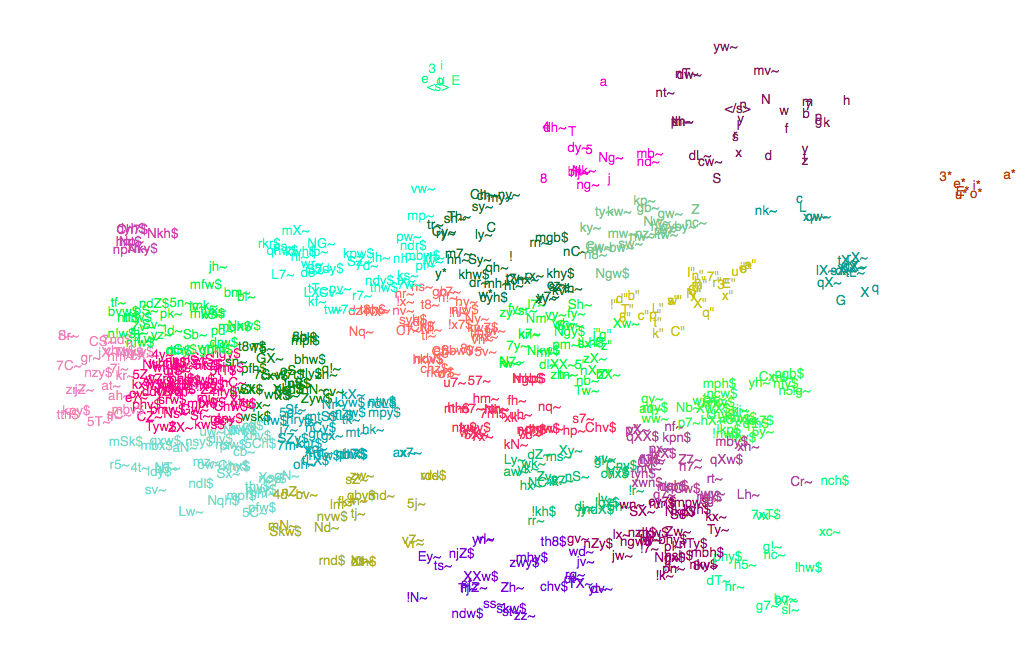
\includegraphics[width=\textwidth]{phoneme_embeddings_overview_ap} 
\caption{t-SNE visualization of the embeddings of all 720 phonemes contained in ASJP, trained with word2vec. The colors represent clusters inferred by Affinity Propagation. The model can clearly separate vowels and various forms of special articulation types. Pulmonic consonants can also be separated clearly from other coarticulation variants, as can uvular or pre-nasalized sounds. Less frequent phonemes, however, cannot be clearly differentiated. }
\label{default}
\end{center}
\end{figure}

\begin{figure}[htbp] %  figure placement: here, top, bottom, or page
   \centering
   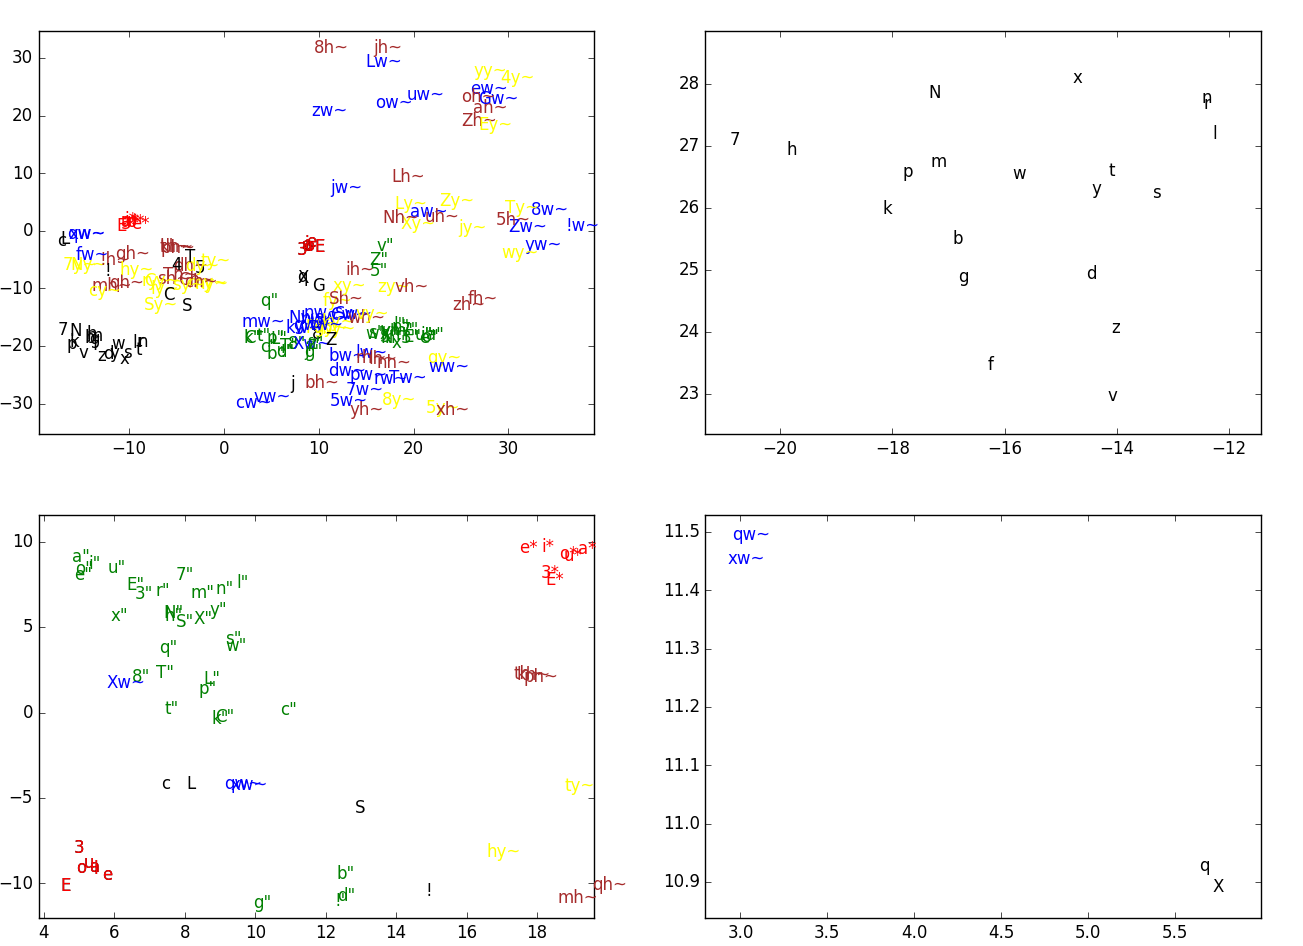
\includegraphics[width=\textwidth]{phoneme_embeddings_word2vec_all.png} 
   \caption{Other t-SNE visualizations of the embeddings created by word2vec. (top left) The model learns to clearly separate natural classes such as vowels, plain pulmonic or glottalized consonants, while other articulations seem to spread over the feature space. The colors indicate membership of a natural phonological class.  (top right) A more detailed view on plain pulmonic consonants. Note the linear dependencies between voiced and unvoiced plosives and their respective nasal variant. (bottom left) Another detailed view. Note how the labialized uvular sounds cluster among glottalized consonants. (top right) The model seems to capture different manners of articulations across articulation type boundaries, as the linear dependency shows here.}
   \label{fig:word2vec_all}
\end{figure}

\subsection{Word Embeddings}

\subsubsection{Autoencoders}
\subsubsection{Variational Autoencoders}

Following this, 4 different models are investigated here:
\begin{enumerate}
\item A model that tries to maximize $p(W=w|z;W)$, i.e. that learns the manifold creating the words as such
\item A model that tries to maximize $p(W=w,C=c|z;W,C)$, i.e. that learns the manifold creating the words and the respective concepts
\item A model that tries to maximize $p(W=w,C=c,G=g|z;W,C,G)$, i.e. that learns the manifold creating the words, the respective concepts and the geographical location
\item A model that tries to maximize $p(W=w|z,C=c;W)$, i.e that learns the manifold creating words given the respective concept.
\end{enumerate}

\subsection{Clustering}
\subsubsection{Affinity Propagation}
\section{Evaluation}
\subsection{Data}
\subsection{Results}
\section{Resume}
\section{Acknowledgements}
For training the phoneme embeddings, I used the word2vec implementations provided by the gensim package \cite{rehurek_lrec}. The Autoencoder was implemented with Keras \cite{chollet2015keras} and Tensorflow \cite{tensorflow2015-whitepaper}. The clustering algorithms used here were provided by scikit-learn \cite{scikit-learn}. All code connected to this thesis can be found on my github \footnote{https://github.com/marlonbetz/BA}
%\subsection{}


\bibliographystyle{apa}
\bibliography{references}
\end{document}  